\subsection{Results} \label{subsection: IPCResults}
Figure~\ref{fig:timeseriesIPC} visualizes the results of the baseline CPC and two IPC controllers, with parameters optimized for 4\,m/s and 13\,m/s pitch rate limits. In all test cases, the turbine is excited with the same wind signal, which has a mean wind speed of 16\,m/s and corresponds to turbulence class~B. The first subplot shows this wind speed signal, which is also used for controller tuning during the optimization. The subsequent plots display generator torque, pitch angles, rotor speed, tower fore-aft acceleration, generator power, and blade root out-of-plane moments.
\begin{figure} [H]
    \subfloat[Pitch rate limit 4\textdegree/s]{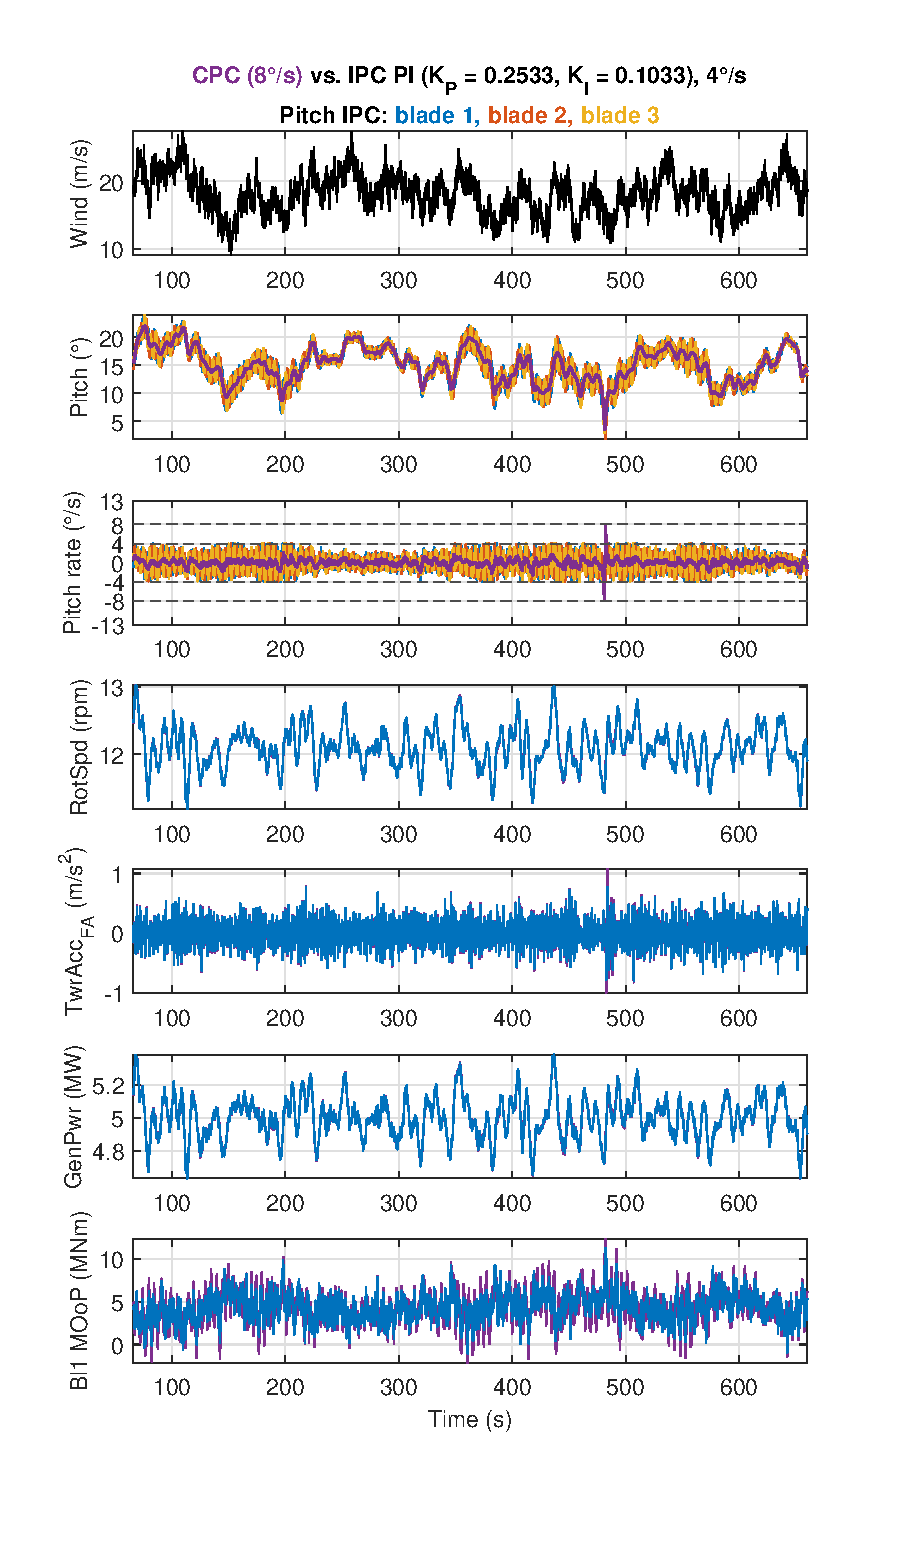
\includegraphics[width=0.49\textwidth]{figures/figures_WESC25/fig00a_Timeseries1.eps}}\hfill 
    \subfloat[Pitch rate limit 13\textdegree/s]{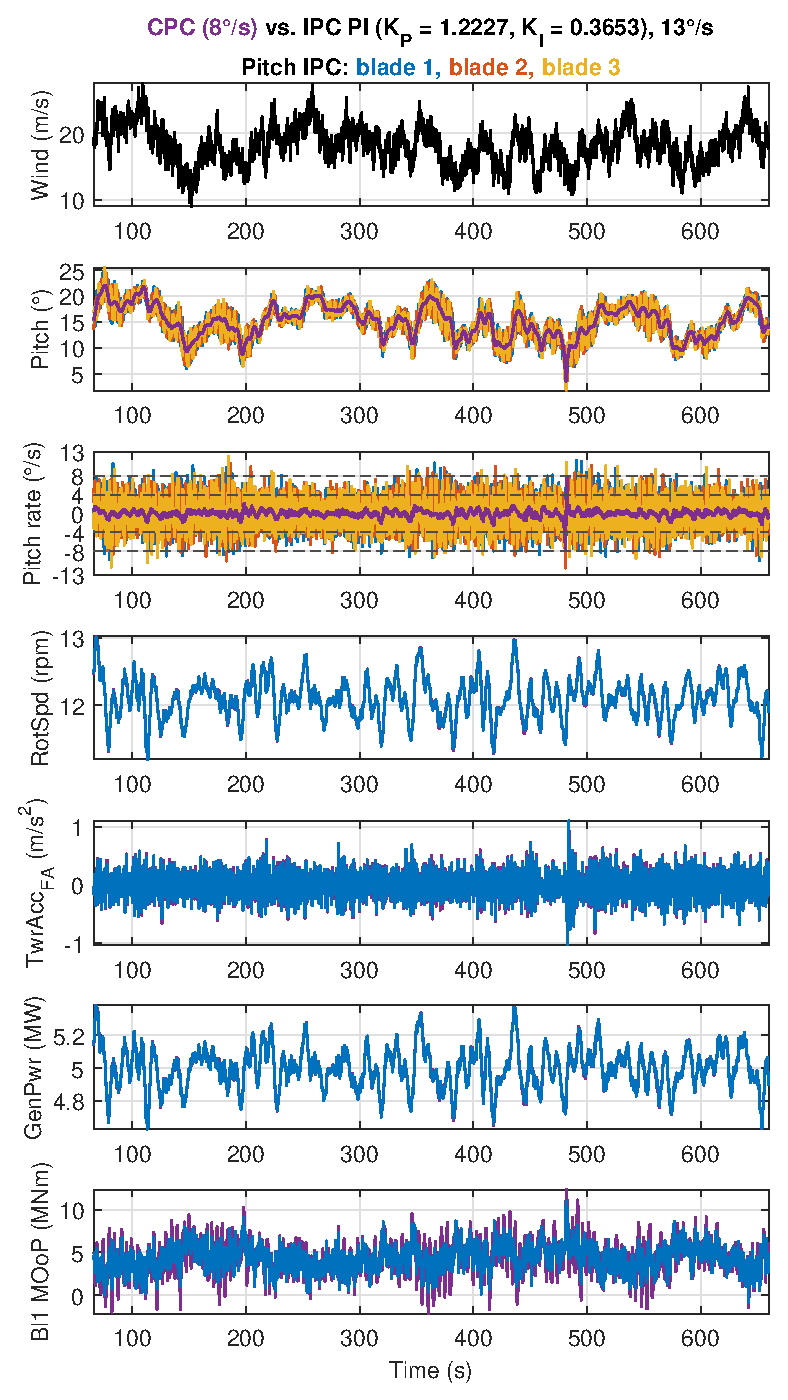
\includegraphics[width=0.49\textwidth]{figures/figures_WESC25/fig00a_Timeseries3.eps}}\hfill
    \caption[Controller comparison: Baseline and IPC PI with different pitch rate limits.]{Controller comparison: Baseline (black) and IPC PI (blue, red and yellow lines pitch signals, blue all other signals) with different pitch rate limits for turbulent wind (16\,m/s mean, IEC turbulence class B (14\%)). Rate limits: Low (4\textdegree/s) and high (13\textdegree/s) for IPC, standard  (8\textdegree/s) for baseline PI. Displayed signals: wind speed, pitch, states, power, and out-of-plane blade root moments.}
    \label{fig:timeseriesIPC}
\end{figure}

Generator torque, rotor speed, and generator power remain nearly unchanged between the two IPC configurations and the baseline PI CPC. This is expected, as the power control logic, which sets the generator torque and collective pitch demand, is identical across all controllers. Differences in tower fore-aft motion are also nearly imperceptible in this time series. The most notable differences appear in the pitch signals, which oscillate at the 1P frequency in both IPC cases, and in the resulting blade root out-of-plane moments. At the lower pitch rate limit of 4\textdegree/s, shown in the left column, the IPC controller has also only a limited effect on the blade root out-of-plane moments. In contrast, the right column, corresponding to the very high pitch rate limit of 13\textdegree/s, shows that the individual pitch actuators significantly reduce the variance of the out-of-plane moments, thereby improving load reduction on the blades. A very slight decrease in tower fore-aft acceleration is also detectable at this rate limit. 
As expected, increasing the allowable pitch rate enhances the effectiveness of the IPC controller in alleviating structural loads.   

Figure~\ref{fig:PSDIPC} shows the Power Spectral Density (PSD) of the blade root out-of-plane moment to visualize and explain the gradual improvement with increasing pitch rate for all three test cases. The black line represents the baseline CPC. The blue line, representing IPC with a 4°/s rate limit, reduces the 1P peak by 87\%, while the red line, representing IPC with an 8°/s rate limit, further lowers it, achieving a significant 98\% reduction. At the 2P frequency, the blue line shows a slight increase compared to the baseline, while the red line effectively lowers the 2P peak. As expected, the 8°/s rate limit offers better load reduction across both 1P and 2P frequencies. The controller tuned with the rate limit set to 13°/s, depicted as a yellow line, decreases the 1P and 2P peaks even more. 
\begin{figure}[h]
    \begin{center}
        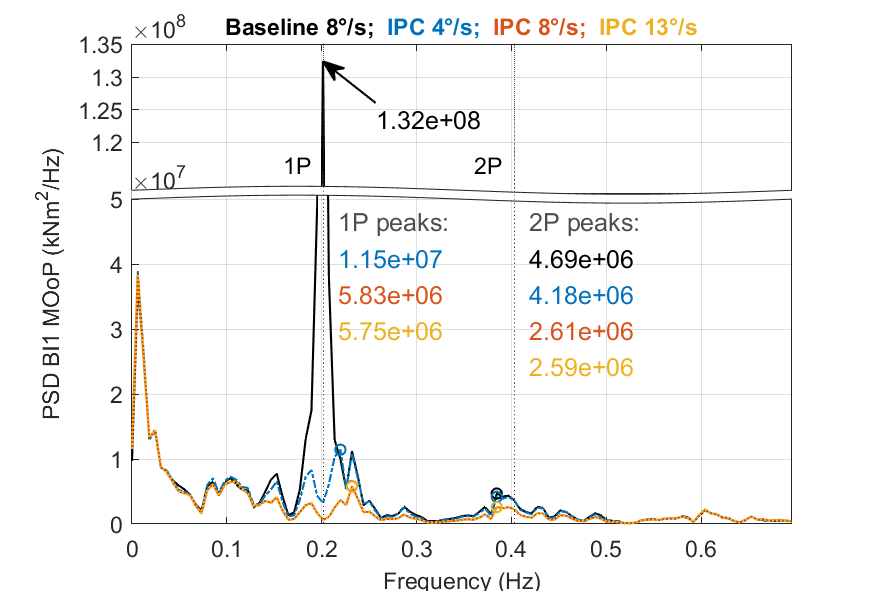
\includegraphics[width=0.6\textwidth]{figures/figures_WESC25/fig02_PSDroot_breaky_ratecomp.png}
        \caption[Controller comparison: Power Spectral Density of blade root out-of-plane moment of baseline PI with 8\textdegree/s rate limit, IPC with 4°/s,  8°/s, and 13°/s rate limit]{Controller comparison: Power Spectral Density of blade root out-of-plane moment of baseline PI (black) with 8\textdegree/s rate limit, IPC with 4°/s rate limit (blue),  8°/s rate limit (red), and 13°/s rate limit (yellow)}
        \label{fig:PSDIPC}
    \end{center}
\end{figure}

Table~\ref{tab:stddev_unified_IPC} summarizes the standard deviation of the signals shown in Figure~\ref{fig:timeseriesIPC} for IPC rate limits of 4°/s, 8°/s, and 13°/s. The baseline PI values are completely insensitive to the rate limit as the pitch rates stay below the limit of 4°/s, they are constant across all three cases. For the states and power output, the introduction of IPC also does not produce any observable effect. Even the tower fore-aft acceleration, which appeared marginally improved under visual inspection at 13°/s, shows a ratio of 1.00 throughout. The pitch rate standard deviation increases unavoidably for the IPC test cases: by 27\% at the most restrictive limit of 4°/s, and by factors of 3.61 and 5.74 at 8°/s and 13°/s respectively. In contrast, the blade root out-of-plane moment is reduced by 5\%, 21\%, and 23\% across the three limits, consistent with the spectral load reductions at 1P and 2P visible in Figure~\ref{fig:PSDIPC}.
\begin{table}[htbp]
    \centering
   \caption[Standard deviation comparison: Baseline PI vs. IPC for turbulent wind with 
   different pitch rate limits.]{Standard deviation of IPC blade pitch rate and blade root 
       out-of-plane moment for turbulent wind with different pitch rate limits. Values in brackets show 
       the ratio to the PI baseline. Tower fore-aft acceleration, generated power, and rotor 
       speed standard deviations are identical to the PI baseline across all rate limits and are 
       therefore omitted. PI baseline standard deviations differ only for the blade pitch rate (0.54\textdegree/s)
       and blade root out-of-plane moment (1628.85\,kNm).}
    \label{tab:stddev_unified_IPC}
    \begin{tabular}{l rrr}
        \toprule
        & \multicolumn{3}{c}{ IPC rate limit (\textdegree/s) (ratio to CPC rate limit (\textdegree/s))} \\
        \cmidrule(lr){2-4}
        Signal & low: 4\textdegree/s & standard: 8\textdegree/s & high: 13\textdegree/s \\
        \midrule
        Tower fore-aft acc.\ (m/s$^2$)  & 0.17 (1.00) & 0.17 (1.00) & 0.17 (1.00) \\
        Generated power (kW)             & 91.59 (1.00) & 91.78 (1.00) & 91.97 (1.00) \\
        Rotor speed (rpm)                & 2.09 (1.00) & 2.09 (1.00) & 2.10 (1.00) \\
        Blade pitch rate (\textdegree/s) & 0.69 (1.27) & 1.95 (3.61) & 3.09 (5.74) \\
        Blade root OoP moment (kNm)      & 1546.19 (0.95) & 1282.12 (0.79) & 1248.97 (0.77) \\
        \bottomrule
    \end{tabular}
\end{table}